\documentclass[10pt,a4paper]{article}
\usepackage[margin=2.1cm]{geometry}
\usepackage{amsmath,amssymb,graphicx,booktabs,hyperref,xcolor,enumitem,float}
\hypersetup{colorlinks,linkcolor=blue!50!black,urlcolor=blue!50!black,citecolor=blue!50!black}
\setlist{itemsep=1pt,topsep=3pt}
\newcommand{\pr}[1]{\href{https://github.com/uwplasma/JAX-in-Cell/pull/#1}{\#{#1}}}
\title{JAX-in-Cell: relativistic collisions, radiation reaction and minimum-power RF runaway control\\[2pt]\large Review note for the stacked pull requests \#75--\#80, with the helicon scattering study (Section~\ref{sec:helicon})}
\author{Rogerio Jorge}
\date{13 November 2026}
\begin{document}
\maketitle
\tableofcontents

\section{Purpose and how to read this note}
This note collects in one place the goals, equations, methods, results and limits of the work that
continues the radiative-control reference, and lists every open pull request with what it does and how to
merge it. All PRs are drafts on \texttt{uwplasma/JAX-in-Cell}; none is merged. Raw data and analysis scripts are in \texttt{results/<lane>/}, each with a \texttt{NOTES.md}. The research log is \texttt{docs/research\_log.md} and the literature survey is in \texttt{docs/literature/}.

\paragraph{Goal.} A slim, fast, differentiable local kinetic capability with validated relativistic
collisions, radiation reaction, prescribed fields and exact work accounting, and with it a defensible
\emph{best-found} minimum supplied RF energy for suppression of a specified energetic-electron population,
with CPU/GPU profiling and a gated quantum-radiation roadmap.

\paragraph{Rules applied throughout.} Extend existing modules (no new production module, no new
dependency); 100\% statement and branch coverage, flake8 on the whole tree and \texttt{sphinx -W};
tests are independent physics or literature checks, never copies of the implementation; physical targets
and gates are never relaxed to obtain a pass; negative results are reported.

\section{Pull requests and merge procedure}\label{sec:prs}
\begin{table}[H]\centering\small
\begin{tabular}{@{}llp{8.6cm}r@{}}
\toprule
PR & Branch & Content & $+/-$ lines\\\midrule
\pr{75} & \texttt{relativistic-radiative-control} & Reference branch: momentum $u=\gamma v$, reduced LL radiation, relativistic COM collisions, prescribed-field callbacks, work ledger, checkpointing, four examples; plus the x64-ordering fix. & 3767/247\\
\pr{80} & \texttt{perf-profile-optimize} & GPU deposition/gather speedups, fix for the NaN gradient on JAX 0.6.2 (Python 3.10), profile tables. & 365/19\\
\pr{77} & \texttt{runaway-baseline} & Collision moment restoration (\texttt{restore=True}), collision validation tests, homogeneous no-RF runaway baseline example. & 613/8\\
\pr{79} & \texttt{rf-minimum-power} & Quasilinear whistler response validated against resolved pushes, explicit source-energy ledger, best-found minimum RF energy example. No production change. & 858/1\\
\pr{78} & \texttt{radiation-references} & Through-pulse reduced vs full LL against the exact plane-wave solution, opt-in \texttt{ll\_full}, collective synchrotron ring formation, mover convergence. & 415/25\\
\pr{76} & \texttt{quantum-recoil} & $\chi$ monitor, LCFA parameter, quantum mean recoil \texttt{ll\_quantum} with $g(\chi)$, gated roadmap. & 294/29\\
\bottomrule\end{tabular}\end{table}

\paragraph{Merge order.} The lane PRs were developed in parallel on top of \pr{75}. Pairwise merge tests
found textual conflicts between \pr{76} and \pr{78} (four files), \pr{76} and \pr{80} (one file), and
\pr{77} and \pr{78} (one file). They have been restacked into a single linear chain
\[
\text{\#42 (research-release)}\leftarrow\pr{75}\leftarrow\pr{80}\leftarrow\pr{77}\leftarrow\pr{79}\leftarrow\pr{78}\leftarrow\pr{76},
\]
each PR's base set to its predecessor, conflicts resolved by keeping both features, and the full gate run
at the top of the stack (Section~\ref{sec:status}). To merge: merge \#42 into \texttt{main} first (or keep
\#75 on \texttt{research-release}), then merge each PR in the order above into its base; GitHub retargets
the next PR automatically when its base branch is merged and deleted. \pr{80} must precede the others
because it carries the Python 3.10 fix that their CI needs. \pr{79} depends on the baseline example in
\pr{77}. Each PR can be stopped at: later PRs are optional additions.

\section{Implemented physics (PR \#75)}
\subsection{Momentum and radiation reaction}
Particles may carry SI specific momentum $\mathbf u=\mathbf p/m=\gamma\mathbf v$. Classical reduced
Landau--Lifshitz radiation (\texttt{Radiation(model="ll\_reduced")}) uses the cancellation-resistant form
with $\boldsymbol\eta=\mathbf u/c$, $\boldsymbol\beta=\boldsymbol\eta/\gamma$,
$\mathbf f=\mathbf E/c+\boldsymbol\beta\times\mathbf B$, $\mathbf h=\boldsymbol\eta\times\mathbf f$,
$S=f^2+h^2$, $\tau=q^2/(6\pi\varepsilon_0 mc^3)$:
\begin{align}
\mathbf a_{\rm RR}&=\tau\Big(\frac qm\Big)^2 c\Big[\mathbf f\times\mathbf B-(\boldsymbol\beta\cdot\mathbf f)(\boldsymbol\beta\times\mathbf B)+(\boldsymbol\beta\times\mathbf f)\times\mathbf f-|\mathbf h|^2\boldsymbol\beta\Big],&
P_{\rm rad}&=\tau\Big(\frac qm\Big)^2mc^2S .
\end{align}
The sum-of-squares form avoids subtracting nearly equal invariants. The explicit mover is a midpoint RK
radiation half-step, a Boris step and a radiation half-step; the implicit mover includes RR in its Picard
residual. Mechanical RR work and emitted energy are separate ledgers: in parallel electric acceleration the
reduced LL force vanishes while Larmor emission is positive.

For a $90^\circ$ electron in uniform $B$ the exact solution is
\begin{equation}
\gamma(t)=\coth\!\big(t/\tau_B+C\big),\qquad \tau_B^{-1}=\frac{e^4B^2}{6\pi\varepsilon_0m^3c^3},
\end{equation}
so $\tau_B=1.290$\,s at 2\,T (independently recomputed). The magnetic-cooling example reaches maximum
relative error $8.6\times10^{-13}$ in $\gamma$.

\subsection{Relativistic binary collisions}
In the relativistic solver, pairs (with odd-cell triplets) scatter elastically in the center-of-momentum
frame with the Pérez (2012) rate and Nanbu cumulative angle, Higginson pair-local density and unequal-weight
acceptance. The per-step scattering parameter is
\begin{equation}
s=\frac{n\,\ln\Lambda\,q_1^2q_2^2\,\Delta t}{4\pi\varepsilon_0^2c^4m_1\gamma_1m_2\gamma_2}\,
\frac{\gamma_{\rm c}\,p^*}{m_1\gamma_1+m_2\gamma_2}\Big(\frac{m_1\gamma_1^*m_2\gamma_2^*c^2}{p^{*2}}+1\Big)^2,
\end{equation}
and the angle is sampled from the Nanbu distribution with $\langle\cos\chi\rangle=\coth A-1/A=e^{-s}$.
Equal weights conserve pair four-momentum to rounding; unequal weights conserve moments in expectation only.
The Coulomb logarithm is mandatory for relativistic runs.

\subsection{Prescribed fields, work ledger, autodiff}
Pure callbacks $(\mathbf x,t,\theta)\mapsto(\mathbf E,\mathbf B)$ with dynamic parameter pytrees add to static
and self-consistent fields. A per-species \texttt{Work} ledger streams kinetic, prescribed, RR, radiated and
collision work (J/m$^2$ in this planar code), and \texttt{energy\_balance} closes the budget. Step
checkpointing lowers reverse-mode residual storage. Collision derivatives are conditional on the random
draws and pairings.

\paragraph{Reference validation (re-checked).} 637 tests, 100\% statements (2838) and branches (726). RF
example AD/FD mismatch $8.3\times10^{-10}$; laser-beam final-$\gamma$ error $1.6\times10^{-8}$; RF
source-control continuum gradient error $3.9\times10^{-4}$ (gate 0.3\%). I fixed one gate failure on this
branch: \texttt{rf\_source\_control.py} set double precision after importing JAX (commit \texttt{0927701}).
CI on \#75 now passes (Python 3.12, 3.13, examples, build).

\section{Literature survey and model choices}
The survey (files \texttt{literature/*.md}) recommends, for each piece, one production model and the
alternative worth a comparison run:
\begin{itemize}
\item Collisions: Nanbu--Pérez with the uncapped Pérez strength, Higginson (2020) for unequal weights;
alternative Angus et al.\ (2025, arXiv:2407.19151) exact energy/momentum restoration (read from the abstract only).
\item Radiation: reduced LL; Niel et al.\ (2018) $g(\chi)$ as an option; full LL, Fokker--Planck and Monte Carlo emission as alternatives.
For 20\,MeV in 2\,T, $\chi\approx2\times10^{-8}$, so quantum corrections are irrelevant to the runaway problem.
\item Runaways: Connor--Hastie critical field, Hesslow (2019) avalanche growth as reference, Embréus (2018) knock-on source.
\item Source power: explicit current-sheet drive with a Poynting ledger.
\item Gradients: pathwise derivatives with pairing indices held fixed; no autodiff through discrete photon emission.
\end{itemize}
Independent test numbers: $\tau_c=4\pi\varepsilon_0^2m^2c^3/(ne^4\ln\Lambda)$ and $E_c=mc/(e\tau_c)$ give, at
$n=10^{18}$\,m$^{-3}$ and $\ln\Lambda=15$, $\tau_c=2.23$\,s and $E_c=7.6\times10^{-4}$\,V/m.
Gaps: some papers read only as abstracts; Rosenbluth--Putvinski and Kennel--Engelmann factors need checking;
no CODE/DREAM numbers were retrieved.

\section{No-RF runaway baseline and collision restoration (PR \#77)}
\subsection{Moment restoration}
After each cross-species collision stage, each cell's weighted momentum and energy are restored to their
pre-stage values by a uniform momentum shift and a Newton-solved scaling of the heavier-weight species'
momenta about their mean; the light species is bit-identical for the same random key. Self-collisions are
not corrected. Default off.
\begin{itemize}
\item 64 realizations: raw energy-defect rms $1.4\times10^{-3}$\,J/m$^3$ $\to$ $4.8\times10^{-13}$ restored.
\item No rate bias: seed collision work $-3.601(18)\times10^{-5}$ raw vs $-3.480(18)\times10^{-5}$ restored.
\item The cold-target defect variance matches the Higginson estimate $2(R-1)/M$ before restoration and is below $10^{-10}$ after.
\item All four reference 64-seed pilots reproduce the documented digits.
\end{itemize}

\subsection{Validation tests added}
Relaxation to Maxwell--Jüttner (temperature and Kolmogorov--Smirnov); electron--ion equilibration against the
exact Spitzer rate ($m_i=25m_e$, $T_e/T_i=4$), kernel exchange 0.98 of exact Spitzer as $\Delta t\to0$;
Higginson defect variance; Connor--Hastie critical force on a $\gamma=100$ electron.

\subsection{Baseline}
Homogeneous 0D3V kinetics: $B=2$\,T, $n=10^{18}$\,m$^{-3}$, $T=100$\,eV, 20\,MeV seed fraction $10^{-5}$,
$\ln\Lambda=15$, total mean field $E=5$\,mV/m held by an ideal $J_{\rm ext}=-J_{\rm plasma}$, with DC work per
species. Compared with a reduced test-particle ODE (drag, pitch scattering, drive, synchrotron):
\begin{table}[H]\centering\small\begin{tabular}{@{}lcc@{}}\toprule
case & kinetic $\Delta\langle\gamma\rangle$ & reduced ODE\\\midrule
100\,$\mu$s, 64 realizations & $-9.864\times10^{-4}$ & $-9.888\times10^{-4}$\\
5\,ms, from $\gamma=40$ & $-4.959\times10^{-2}$ & $-4.935\times10^{-2}$\\
5\,ms, from $\gamma=5$, pitch 0.3 & $+3.23\times10^{-3}$ & $+3.32\times10^{-3}$\\\bottomrule
\end{tabular}\end{table}
Bulk Ohmic power 32--37\,W/m$^3$ against the Spitzer estimate of about 32.

\paragraph{Key physics result.} With $E/E_c=6.5$, synchrotron drag creates a stable fixed point at
$\gamma_{\rm eq}=13.13$ (6.2\,MeV). The 20\,MeV seed decays (1/e time 4.64\,s) instead of running away, and a
suppressed tail regrows slowly (Fig.~\ref{fig:regrowth}). In this scenario minimum-RF suppression is degenerate.
Neglected terms, bounded: avalanche $\le3.5$\%/s, bremsstrahlung $\approx0.2$\% of $eEc$, no Dreicer source,
no screening for $Z=1$.

\paragraph{Correction made during review.} The first version quoted a thermal collision rate of
$5\times10^6$\,s$^{-1}$; the Braginskii value is $\tau_e=23\,\mu$s ($4.4\times10^4$\,s$^{-1}$). The claimed
10$\times$ Ohmic overestimate at $\Delta t=2\,\mu$s was inferred from that wrong rate, never measured;
measurements show no resolvable $\Delta t$ effect. The 0.2\,$\mu$s step ($\tau_e/115$) is a convergence
choice for slow electrons; 1--2\,$\mu$s suffices for seed quantities. Fixed in commit \texttt{37ef059}.
\begin{figure}[H]\centering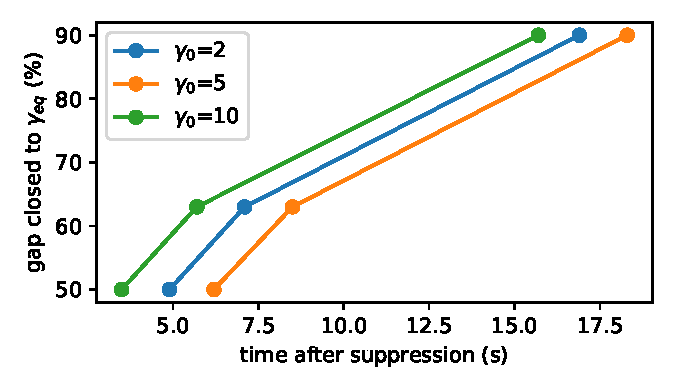
\includegraphics[width=.55\textwidth]{fig/l2_regrowth.pdf}
\caption{No-RF regrowth after suppression to $\gamma_0$: time to close 50/63/90\% of the gap to $\gamma_{\rm eq}$ (reduced ODE; first points confirmed kinetically within 3\% at 5\,ms).}\label{fig:regrowth}\end{figure}

\section{Minimum supplied RF energy (PR \#79)}
\subsection{Scenarios}
\begin{enumerate}
\item \textbf{Reference scenario ($E=5$\,mV/m):} bounded negative result. All suppressed starts peak below
10\,MeV; minimum RF is zero. The fixed point never disappears; it crosses 10\,MeV at $E=6.26$\,mV/m.
\item \textbf{Declared study scenario ($E=15$\,mV/m):} a numerical choice, not a device prediction.
$E/E_c=19.6$, fixed point 58\,MeV; RF window 0.3\,s, RF-off hold 2.70\,s (measured regrowth from $\gamma=5$ to 10\,MeV), horizon 3.0\,s.
Without RF, the fraction above 10\,MeV grows from 22\% to 100\%. Collision and radiation strengths unchanged.
\end{enumerate}

\subsection{Slow RF response}
Counter-propagating cold right-hand whistler, normal-Doppler resonance
\begin{equation}
\omega-k_\parallel v_\parallel=-\Omega/\gamma ,
\end{equation}
with quasilinear diffusion along the wave-frame invariant $\mathcal E+|v_{\rm ph}|p_\parallel=$ const.
Each test particle sees its own random-phase realization. Checks against resolved Boris windows:
\begin{itemize}
\item wave-force amplitude to 0.7\%;
\item nine held-out in-domain cases: pitch-variance growth ratio (resolved/QL) 0.92--1.67, mean 1.30; mean energy shift 1.1--2.0$\times$ larger when resolved, same sign;
\item out of domain: sparse lines (energy shift changes sign), very dense lines (ratio 0.47), coherent one- or three-line cases (trapping, no diffusion).
\end{itemize}
Validity domain: noise-like band of at least 32 lines at overlap parameter 3, particle inside the band,
$D_{\max}\Delta t\le0.01$; otherwise fall back to the resolved push. The two are never applied together.

\subsection{Source ledger}
Explicit drive current $J_{\rm drive}=\nabla\times\mathbf B/\mu_0-\varepsilon_0\partial_t\mathbf E-J_{\rm plasma}$,
\begin{equation}
P_{\rm src}=-\int J_{\rm drive}\cdot\mathbf E\,dx,\qquad Q_+=\int\max(P_{\rm src},0)\,dt ,
\end{equation}
with zero-crossing quadrature; $Q_+$, returned $Q_-$ and net energy are reported separately for an ideal
nonrecovering port. Ramp closure $10^{-6}$; supplied energy converged to $<10^{-6}$ under refinement; steady
power within 3\% of the closed form. For circular waves there is no cycle-level reactive sloshing; the
dominant cost is energy taken by the resonant tail.

\subsection{Optimization and frozen-control verification}
240 slow-model evaluations per strategy; frozen controls checked on 8192 independent seeds, $\Delta t/2$,
doubled nodes and $\pm30$\% amplitude.
\begin{table}[H]\centering\small\begin{tabular}{@{}lccc@{}}\toprule
strategy & feasible & verified $Q_+$ (J/m$^3$) & fraction $>10$\,MeV at end of hold\\\midrule
no RF & -- & -- & 1.00\\
single band & 2/240 & 8.2 & 0.24\%\\
3 bands, random search & 2/240 & 9.0 & 0.24\%\\
3 bands, evolution strategy & 107/239 & \textbf{5.1} & 1.6\% (95\% upper bound 1.8\%)\\\bottomrule
\end{tabular}\end{table}
\begin{figure}[H]\centering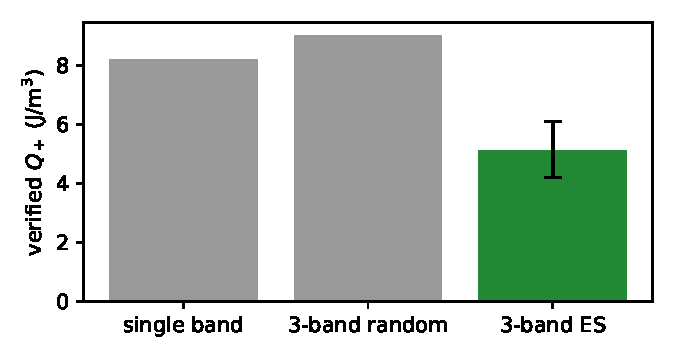
\includegraphics[width=.5\textwidth]{fig/l4_strategies.pdf}
\caption{Verified supplied energy by strategy; bar on the best: amplitude $\pm30$\% check range.}\end{figure}
Best found: 5.1\,J/m$^3$ over 0.3\,s ($4.2$--$6.1$ over the amplitude checks; about 9 if the QL tail exchange
is low by the measured factor 1.0--1.7). For scale, the DC Ohmic work over 3\,s is about 1\,kJ/m$^3$.

\paragraph{What did not hold up.}
\begin{itemize}
\item Suppression is not sustained: controls park the tail near 9\,MeV; with RF off, 34--73\% exceed
10\,MeV after a further 0.5\,s and 100\% after 1\,s.
\item With 2\,s added to the hold, none of 720 evaluations is feasible: a bounded negative result for a 0.3\,s, three-band, $b\le10^{-5}$ window.
\item The best control fails the $-30$\% amplitude check (2.6\%): thin margin.
\item Not modeled: avalanche, bremsstrahlung, transport, antenna coupling, wall-plug efficiency, PIC-level whistler confirmation, CODE/DREAM comparison.
\end{itemize}

\section{Classical radiation references (PR \#78)}
\begin{itemize}
\item \textbf{Through-pulse LL:} reduced and full LL compared with Di Piazza's exact plane-wave LL solution;
the closed form agrees with an independent DOP853 integration to $2.7\times10^{-13}$ of $a_0$. Each model
converges at second order (ratio 4.00). Default beam ($\gamma_0\approx80$, $a_0=15$): model gap
$2.6\times10^{-6}$ of $a_0$, ten times below integration error, so the derivative term is invisible. Strong
stress beam ($\gamma_0=3\times10^4$, $\chi\le0.19$): gap $8.9\times10^{-4}$, resolved by \texttt{ll\_full}.
\item \textbf{\texttt{Radiation(model="ll\_full")}:} opt-in, 41\% extra cost, explicit solver, periodic
boundaries and no sources (enforced). Separate commit, easy to drop.
\item \textbf{Synchrotron ring formation} (Bilbao \& Silva, PRL 130, 165101): 200k markers, self-consistent
fields. PIC ring radius matches exact LL evolution of the same markers within 1\%; their Eq.~7 is 8--12\%
below for $t\ge1.5t_R$, as its assumption predicts. Population inversion $f(p_R)/f(\text{core})=9.2$ at $3t_R$.
$B=10^5$\,T is a chosen value for a short run.
\item \textbf{Movers:} both second order; at equal step the explicit $\gamma$ error is $\sim6\times10^5$
smaller than implicit; radiation substeps reduce energy error only, not gyrophase; Picard saturates in 3 iterations.
\end{itemize}
\begin{figure}[H]\centering
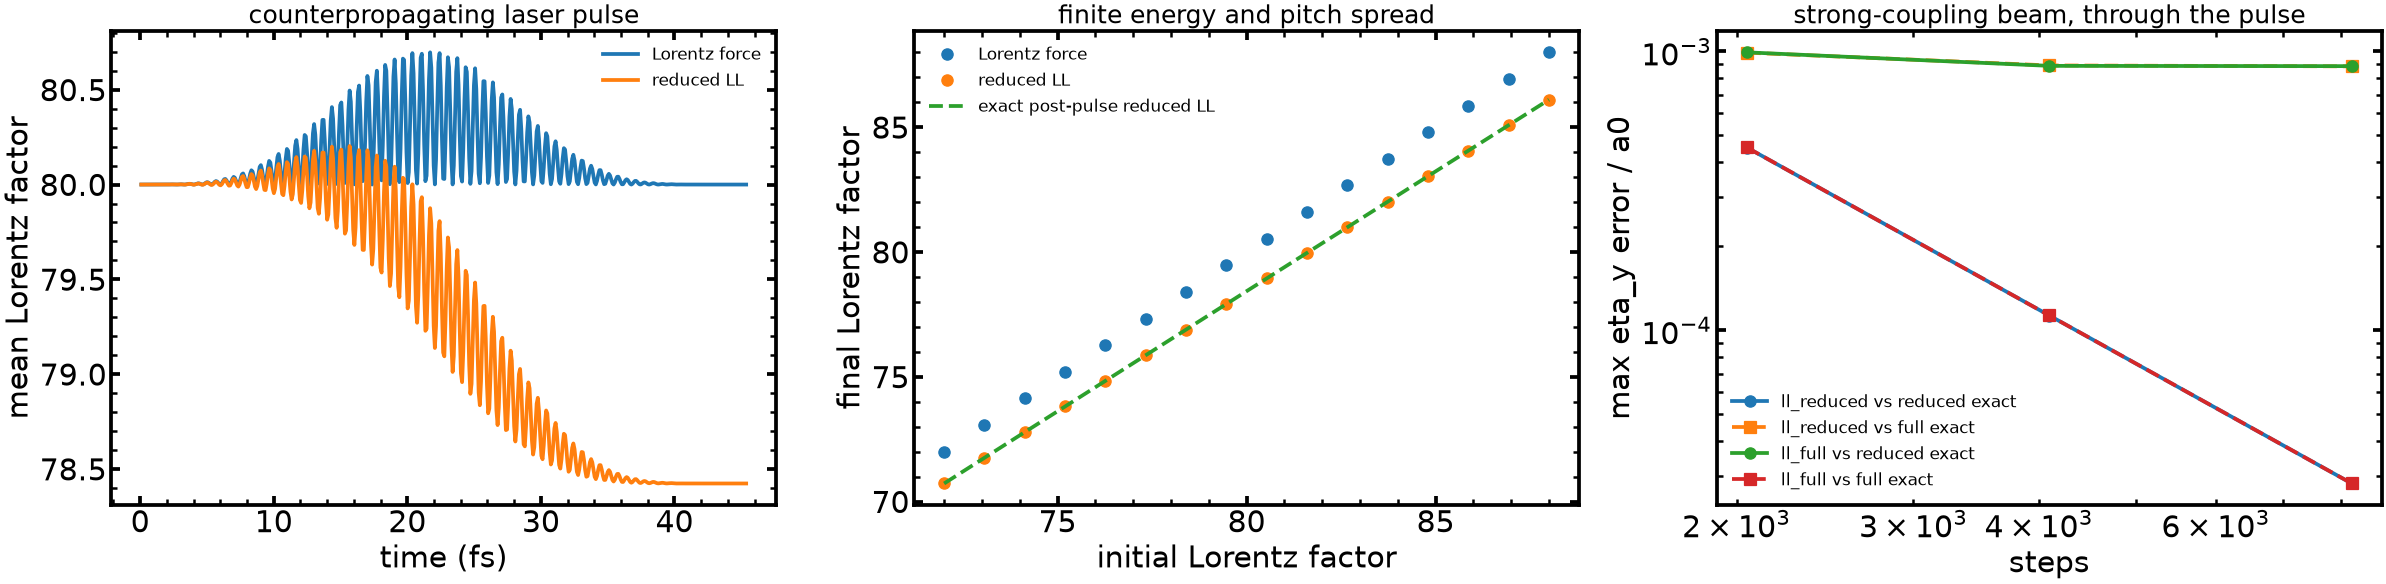
\includegraphics[width=.48\textwidth]{fig/beam_laser_models.png}\hfill
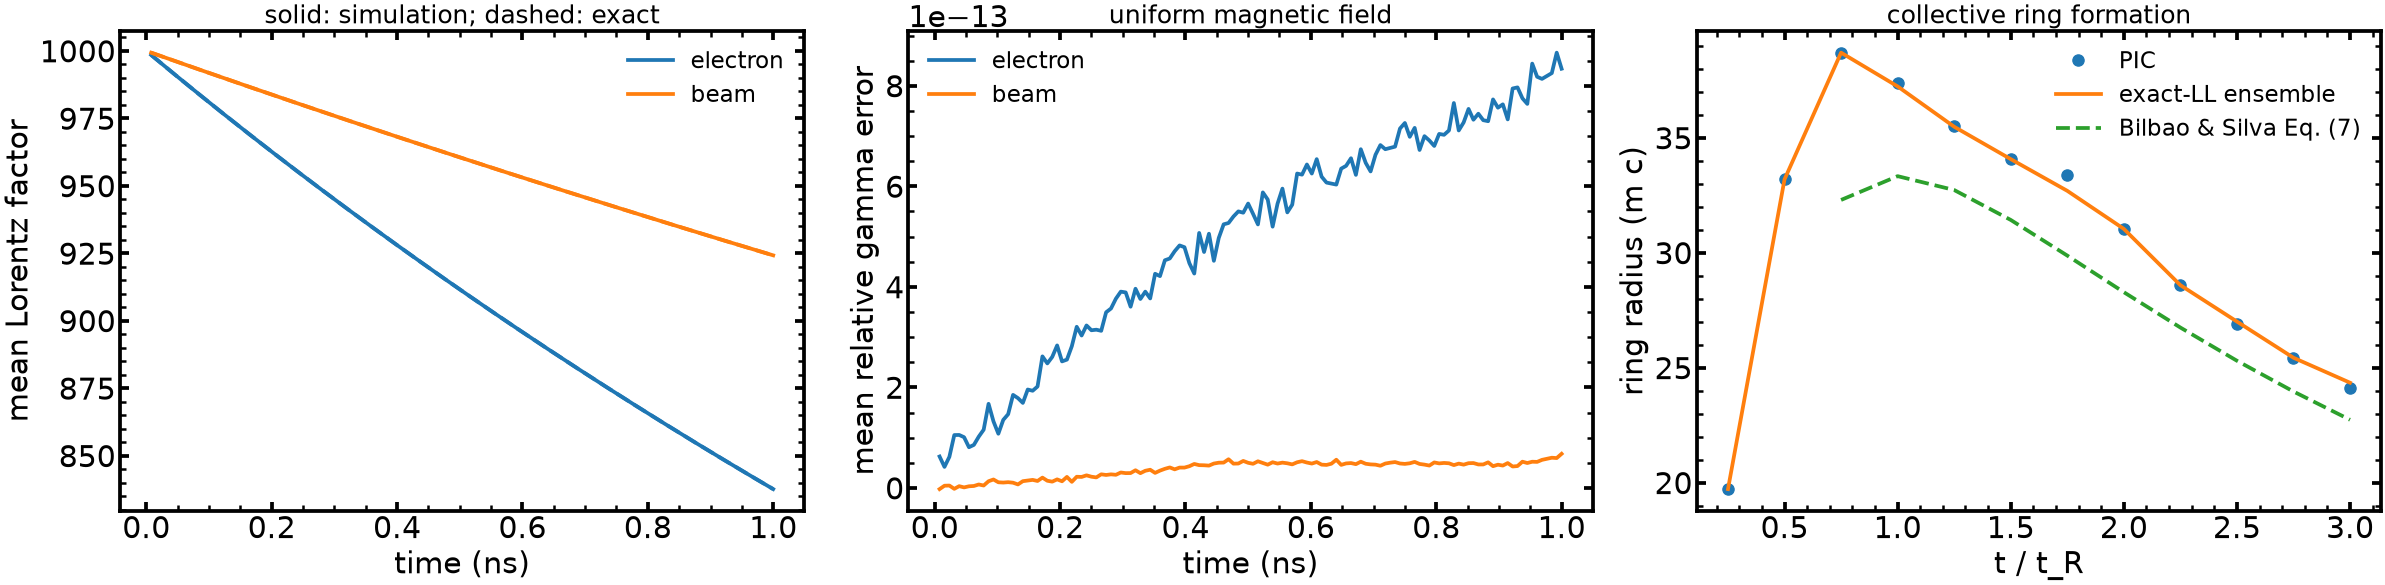
\includegraphics[width=.48\textwidth]{fig/electron_cooling_ring.png}
\caption{Left: reduced vs full LL through the pulse against the exact solution. Right: synchrotron ring formation (PR \#78 figures).}\end{figure}

\section{Quantum radiation stage (PR \#76)}
$\chi=\gamma\sqrt{(\mathbf E/c+\boldsymbol\beta\times\mathbf B)^2-(\boldsymbol\beta\cdot\mathbf E/c)^2}/B_S$
(computed from the same kernel invariant), an emission-weighted mean $\chi$ in the diagnostics and the LCFA
parameter $a=\chi mc^2/(\hbar\omega)$. \texttt{Radiation(model="ll\_quantum")} scales force and emitted power by
\begin{equation}
g(\chi)=\big[1+4.8(1+\chi)\ln(1+1.7\chi)+2.44\chi^2\big]^{-2/3}\qquad\text{(Niel et al.\ 2018)} .
\end{equation}
Validation against independent quadrature of the synchrotron spectrum: $g$ within 1.4\% for
$10^{-6}\le\chi\le10^3$; $dg/d\chi$ within 8.6\% (the fit slope at $\chi\to0$ is $-5.44$ vs exact
$-55\sqrt3/16=-5.954$, stated in the PR); simulated quantum/classical emitted energy equals $g(\chi)$ to
$10^{-3}$ for both movers; $d\gamma/dB$ matches finite differences to $10^{-6}$. Fokker--Planck diffusion,
stochastic emission and pairs are documented with gates but not implemented.
\begin{figure}[H]\centering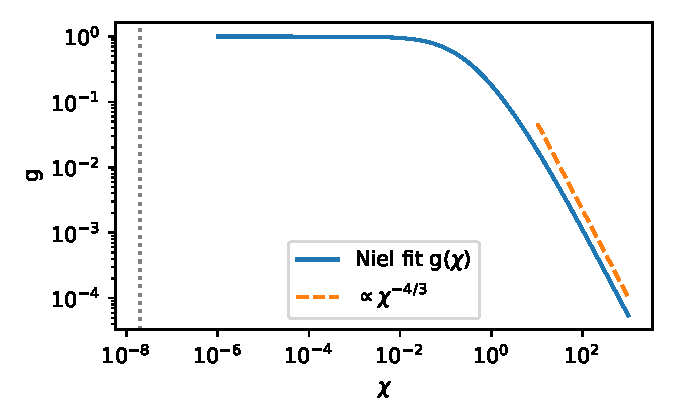
\includegraphics[width=.48\textwidth]{fig/l5_gchi.pdf}
\caption{$g(\chi)$; dotted line: runaway regime $\chi\approx2\times10^{-8}$.}\end{figure}

\section{Performance (PR \#80) and adjacent codes}
\subsection{Gate and Python 3.10 fix}
Office CPU, Python 3.12, JAX 0.12: 642 tests, 0 failures, coverage 100\% of 2862 statements and 734 branches;
flake8 and \texttt{sphinx -W} clean. The NaN gradient on JAX 0.6.2 (the newest JAX for Python 3.10) came
from the reverse pass of a \texttt{lax.cond} in the wall-contact refinement; where the predicate is true
for every particle the refinement is now called directly. Python 3.10: 553 passed, 1 skipped.

\subsection{Optimizations}
Traces (131k electrons, 256 cells, float64): deposition scatter-add 52\% of explicit kernel time, scatters
37\% of implicit, radiation compute-bound, collisions launch-bound. Applied on accelerators: one 3-column
scatter for $\rho,J_y,J_z$; above 8192 particles, 32 private grid copies for deposition and lane-split gather
(so its transpose is also lane-split). CPU keeps the old path (unchanged within 1\%). Derivatives unchanged
to $10^{-12}$. No Pallas kernel (no trace evidence).
\begin{figure}[H]\centering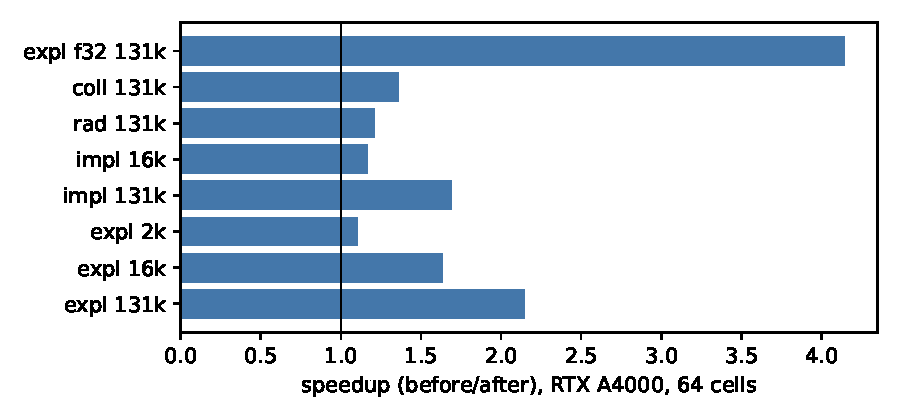
\includegraphics[width=.62\textwidth]{fig/l1_speedup.pdf}
\caption{Before/after GPU forward-time ratio (RTX A4000, shared host, median of alternating fresh processes).}\end{figure}
\begin{table}[H]\centering\small\begin{tabular}{@{}lcc|lcc@{}}\toprule
case (forward) & before & after & case (16k, derivative) & before & after\\\midrule
explicit 131k & 108 & 50.3 & explicit JVP & 26.6 & 15.1\\
implicit 131k & 1550 & 916 & explicit reverse & 32.9 & 24.8\\
collisions 131k & 226 & 166 & implicit JVP & 315 & 250\\
radiation 131k & 375 & 310 & implicit reverse & 820 & 766\\
explicit f32 131k & 60.9 & 14.7 & radiation reverse & 67.7 & 61.5\\\bottomrule
\end{tabular}\caption*{Times in ms. Maintained sheath (6000 steps): 555\,s on one CPU core, 30\,s on GPU. Checkpointing cuts compiler temporary bytes for implicit reverse at 16k from 10.5\,GB to 426\,MB.}\end{table}
Limits: shared GPU throughout; collision loop and radiation untouched; implicit step still 10--15$\times$ explicit;
no multi-GPU comparison.

\subsection{ESSOS and SOLVAX (no PRs)}
ESSOS: GPU loses to CPU below about 128 particles; reverse costs 10--30$\times$ forward; adaptive traces lack
JVP and differentiated traces cannot be sharded; forward sharding peaks at 2.1$\times$ (per-call recompilation,
step-count imbalance). SOLVAX: tridiagonal solves $\sim10^3\times$ faster than dense with adjoints exact to
$4\times10^{-16}$, but in a JAX-in-Cell-like implicit step the field solve is not the bottleneck, and
\texttt{root\_solve}'s dense tangent makes implicit gradients 3--350$\times$ slower than unrolled Picard.
Recommendation: no SOLVAX dependency. Candidate ESSOS PRs (jit reuse, step-balanced sharding, JVP path) need measurement first.

\section{Validation status}\label{sec:status}
\begin{table}[H]\centering\small\begin{tabular}{@{}lp{11.5cm}@{}}\toprule
PR & status\\\midrule
\#75 & GitHub CI green (3.12, 3.13, examples, build).\\
\#80 & full gate on office: 642 passed, 100\% coverage; Python 3.10: 553 passed (\texttt{test\_api.py} excluded for time); examples not rerun.\\
\#77 & 646 passed, 2 base failures since fixed (\#75 x64, \#80 NaN); 100\% coverage.\\
\#79 & no production change; flake8, sphinx, example-name and quick runs pass; full pytest not rerun.\\
\#78 & 639 passed before rebase, 100\% coverage; full suite not rerun after rebase.\\
\#76 & 100\% coverage; one test expectation edited and not rerun on office.\\
stack & all six PRs MERGEABLE. Top (\#76, 200567b) on office CPU: TOTAL 2931 statements, 744 branches, 0 missed (100\%), 0 skipped (openpmd-api, scipy installed), 0 failures; flake8 0 on every branch from \#80 up. \texttt{sphinx -W}: 8 \texttt{dataclasses.replace} docstring warnings under Python 3.10, identical on \#75, so not from the stack. Intermediate branches not re-tested. Restack added one commit on \#76 fixing the merged \texttt{landau\_lifshitz} signature (keyword \texttt{derivative}).\\\bottomrule
\end{tabular}\end{table}
CI on the lane PRs reports only one check because the workflow runs on PRs to \texttt{main}; each will be
fully tested once its base is merged.

\section{Completion against the reference definition}
\begin{table}[H]\centering\small\begin{tabular}{@{}lp{12cm}@{}}\toprule
goal & state\\\midrule
Core physics/API & done; 100\% gate; unsupported combinations rejected.\\
Relativistic collisions & rates, Maxwell--Jüttner, Spitzer, conservation, variance, restoration done; AD qualified as conditional.\\
Radiation and movers & exact magnetic/plane-wave references, full vs reduced LL, convergence and Picard done.\\
No-RF baseline & done with reduced-ODE reference and bounded neglected terms; \textbf{missing} CODE/DREAM comparison.\\
Reduced RF response & held-out validation, coherent limits, no double counting; \textbf{missing} PIC-level whistler window.\\
Minimum supplied resource & best-found 5.1\,J/m$^3$ for the declared horizon; \textbf{sustained} suppression is a bounded negative result.\\
Performance & CPU and single-GPU forward/AD/memory profiles; \textbf{missing} multi-GPU scaling.\\
Examples/docs & consolidated examples, compressed figures, docs updated in each PR.\\
Quantum roadmap & monitor, mean recoil, gated plan done; stochastic stages not implemented by design.\\\bottomrule
\end{tabular}\end{table}


\section{Helicon/whistler scattering of runaways: final conclusions}\label{sec:helicon}
This section summarizes the physics study that followed the PR work (work packages P1--P3 and steps 1--3 in
\texttt{docs/research\_log.md}; data and per-step \texttt{NOTES.md} in \texttt{results/\{P1,P2,P3,step1,step2,step3,pinning,codes\}}).
None of it is in a pull request: it uses the \#77 collision/radiation kernels and a separate full-orbit Boris
integrator, and all scripts and data stay in \texttt{results/}. The question was whether a launched comb of
toroidal helicon lines scatters runaway electrons at a rate set by resonance-island overlap, and whether that
explains the DIII-D helicon power threshold (Choudhury et al., PPCF 68, 105047). The answer is mostly negative for a coherent comb.

\subsection{Baseline against kinetic references (P1, PR \#77 text)}
With the bulk held fixed, the tail of the 0D3V runs ($B=2$\,T, $E=5$\,mV/m, $n\ln\Lambda=1.5\times10^{19}$\,m$^{-3}$, $E/E_c=6.54$)
settles in tens of seconds to a distribution with mode $\gamma=17.65$ (DREAM kinetic 16.8--17.1), pitch 0.101--0.105\,rad
(DREAM 0.106) and mean $\gamma$ within 4--5\% of DREAM after its $p<40$ cut; Richardson extrapolation in the grid reduces the
mean offset to 0.9--2.7\%. A pitch-noise scan moves the mode from the ODE value 13.16 (no noise) to 17.4 (full Ito noise).
The synchrotron fixed point $\gamma=13.13$ of the \#77 baseline is therefore a property of the noise-free test-particle ODE, not a
bound on the kinetic tail; the \#77 wording (``no runaway above 6.2\,MeV'') needs the replacement text drafted in \texttt{results/P1/NOTES.md}
section 4. The avalanche rate cannot be measured, because the collision kernel has no large-angle source. At $E/E_c=6.54$ the
reference rates are DREAM 0.053, CODE 0.073 and Rosenbluth--Putvinski 0.073\,s$^{-1}$; the earlier 0.03\,s$^{-1}$ estimate was about 2$\times$ low.

\subsection{Single line, comb overlap and transient chaos (P2, P3, step 1)}
All amplitudes below are $b=\delta B/B_0$ of one line. A coherent single line departs from quasilinear (QL) diffusion at
$\omega_b^2/|\dot\delta|\approx2$--3, which is $b\sim3.5\times10^{-9}$ for the DIII-D acceleration sweep; at DIII-D amplitudes
($3\times10^{-5}$--$5\times10^{-3}$) the island passage scatters less than QL ($D_{\rm eff}/D_{\rm QL}\sim10^{-5}$--$10^{-3}$, extrapolated from
$\lambda\le10^3$ time compression; the physical case was not run). For two lines the transport jump follows the Chirikov parameter
$\sigma=2(\omega_{b1}+\omega_{b2})/\Delta\omega$, with the jump at $\sigma_c=0.8$--1.0. For the DIII-D toroidal comb (spacing $1/R_0$) the
stationary $D_{\rm eff}/D_{\rm QL}$ of $N=5$--10 lines collapses on $\sigma$, with the 50\% point at $\sigma=0.97$--1.12,
$b_{\rm thr}=1.0\times10^{-4}$ per line (0.6--1.6$\times10^{-4}$), and $b_{\rm thr}\propto\Delta^{1.88\pm0.15}$. Collisions and radiation reaction
do not move the threshold at DIII-D, since $\nu_{\rm eff}/\omega_b\sim10^{-6}$. This is the P3 result, and it holds only on short windows.

Step 1 found two things. The reduced model had lacked the tangential phase term, and with it fixed it agrees with full-orbit
passage to 4--14\%; the earlier $\sigma=2.2$ ``capture'' is a deterministic surfing lag of $\Delta\gamma\approx-0.24$, not trapping. More important,
for a coherent finite comb the motion is bounded chaos: $\langle\Delta\gamma^2\rangle$ rises, fills the line band quickly and then stops, at every
$\sigma$ from 1 to 4. The overlap threshold describes transient diffusion over tens of beat periods (1--10\,$\mu$s), not a steady rate.

\subsection{Phase decorrelation (step 3)}
Independent random-walk phase noise (Lorentzian lines of half-width $\Gamma_\phi$) was added to each of $N=10$ lines of the reduced model.
Window 1000 beat periods (3000 as a check), $\sigma=0.5$--4, $\Gamma_\phi/\Delta\omega=0$--3, 3 seeds of 64 particles. The measure
is the late growth rate of $\langle\Delta\gamma^2\rangle$ relative to the QL prediction for the same finite band, $s_{\rm late}$, together with the fill
$\langle\Delta\gamma^2\rangle/(L_w^2/6)$, where $L_w$ is the band width in $\gamma$ and 1 is complete mixing (Fig.~\ref{fig:s3map}--\ref{fig:s3rate}).
\begin{itemize}
\item At $\Gamma_\phi=0$, $s_{\rm late}=0.00$--0.06 for every $\sigma$. The coherent comb plateaus at fill 0.5--0.7 and stays there to 3000 periods.
\item $s_{\rm late}$ turns on at $\Gamma_\phi/\Delta\omega\approx0.01$--0.03 (0.01--0.4) and reaches the QL value at about 0.1--0.3; a rough law is
$s_{\rm late}\approx\min(1,\,7\Gamma_\phi/\Delta\omega)$, so sustained QL scattering needs a coherence time of a few beat periods or less ($\Gamma_\phi\gtrsim0.14\,\Delta\omega$).
\item The dependence on $\sigma>0.5$ is weak. Overlap sets how fast the band fills (0.5 of complete mixing in 266, 13, 5 and 1 beat periods at $\sigma=1$, 1.5, 2, 3), not whether growth continues.
\item Correction to step 1: in a finite band, QL diffusion also has zero late slope, so a small $D_{\rm eff}/D_{\rm QL}$ at $10^3$ periods is not by itself non-QL. The plateau fill is the discriminator.
\end{itemize}
\begin{figure}[H]\centering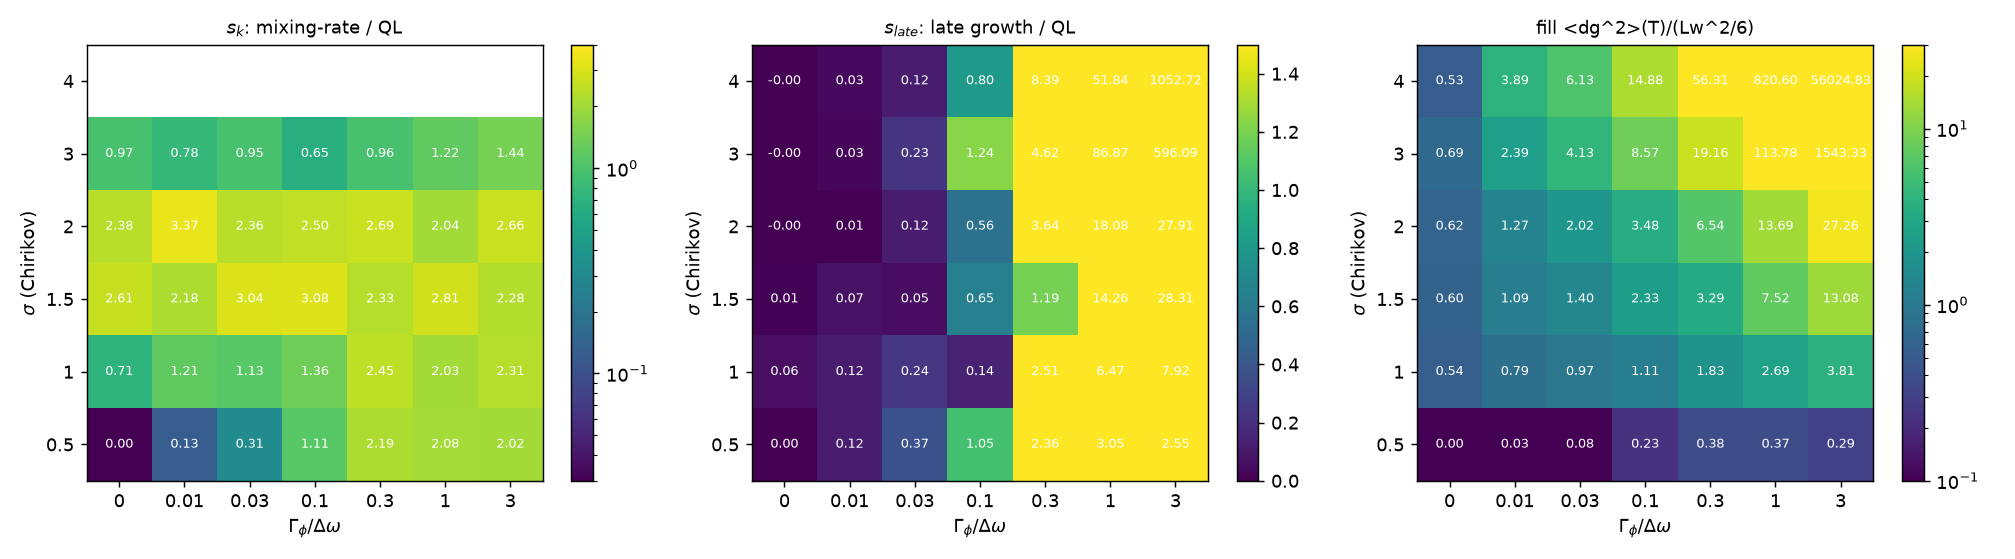
\includegraphics[width=\textwidth]{fig/s3_map.png}
\caption{Step 3 maps over $\sigma$ and $\Gamma_\phi/\Delta\omega$: mixing rate $s_k$ relative to QL (left), late growth relative to QL $s_{\rm late}$ (middle; cells with fill $>2$ are unreliable), fill at $T=1000$ periods (right).}\label{fig:s3map}\end{figure}
\begin{figure}[H]\centering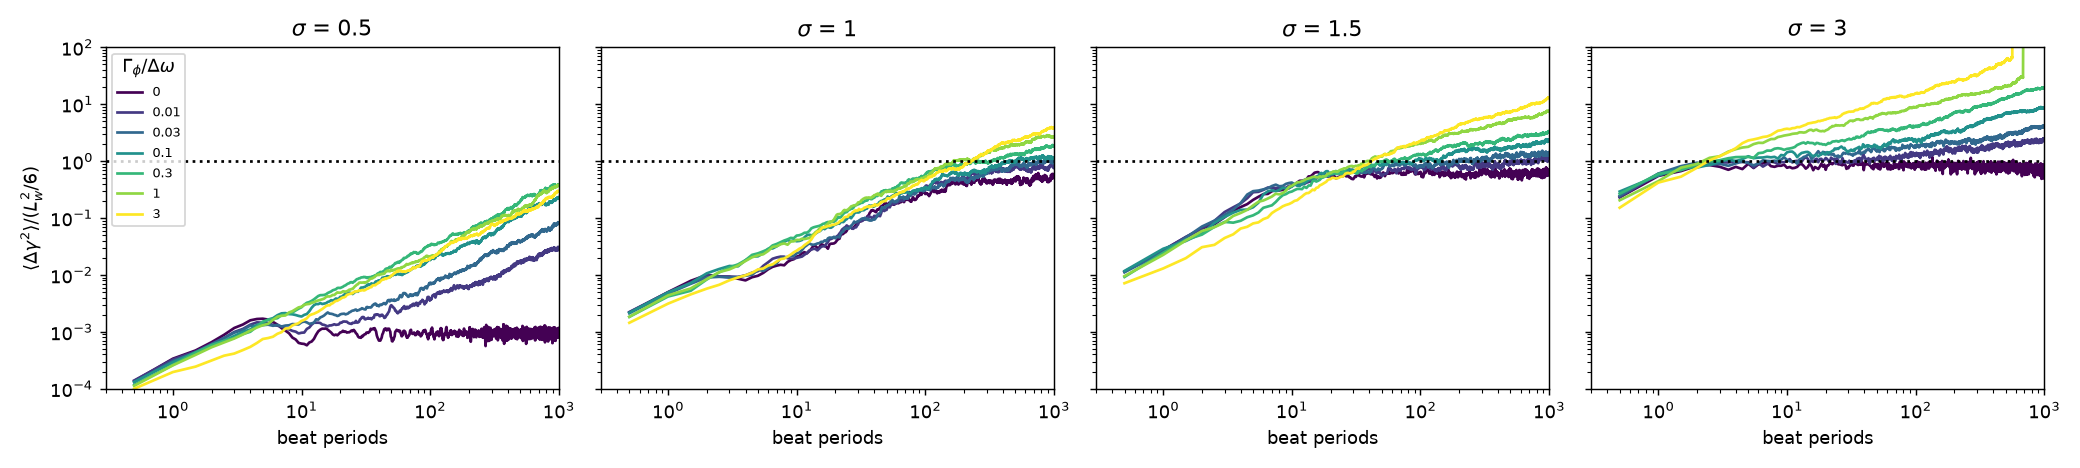
\includegraphics[width=\textwidth]{fig/s3_time.png}
\caption{$\langle\Delta\gamma^2\rangle/(L_w^2/6)$ against time in beat periods. The coherent curve ($\Gamma_\phi=0$) flattens; noisy curves pass the dotted line (complete mixing) and keep growing.}\label{fig:s3time}\end{figure}
\begin{figure}[H]\centering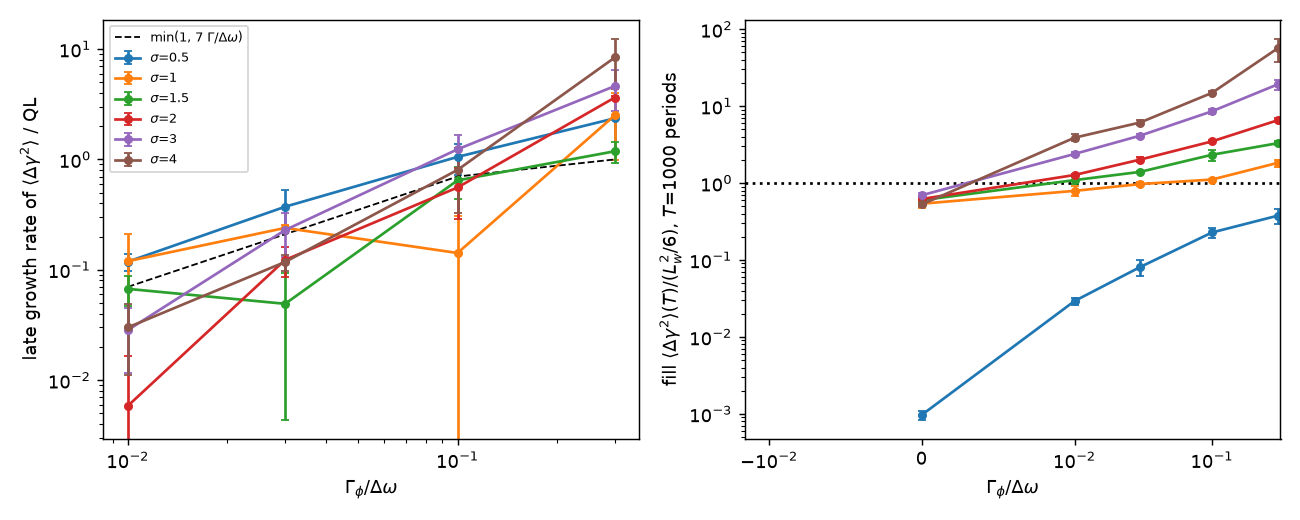
\includegraphics[width=\textwidth]{fig/s3_rate.png}
\caption{Left: $s_{\rm late}$ against $\Gamma_\phi/\Delta\omega$ with the rough law (dashed); error bars are the seed standard error. Right: fill at $T=1000$.}\label{fig:s3rate}\end{figure}

\subsection{Where DIII-D sits}
Step 2 (cold-tensor Landau and TTMP damping, $\Gamma_P$ median $2.7\times10^5$\,s$^{-1}$, 95\% range $4\times10^4$--$1.4\times10^6$) gives
$b/b_{\rm thr}$ medians 0.39, 0.52 and 0.69 at 43, 76 and 150\,kW, so $\sigma\approx0.6$--0.8, with probability of exceeding threshold 6, 17 and 24\%,
and a median threshold power of 280\,kW (75--730\,kW). The source linewidth is Hz to kHz for a phase-locked 476\,MHz klystron, and common-mode noise does not decorrelate lines;
multipass supplies frozen random phases, not decorrelation. My estimate of plasma phase noise gives $\Gamma_\phi/\Delta\omega\sim10^{-6}$--$3\times10^{-2}$, nominally $10^{-4}$--$10^{-3}$ (no measurement).
Only parametric-decay broadening at 8\,MHz spacing (up to 0.3\,$\Delta\omega$, uncalibrated) or deliberate frequency modulation could reach the sustained regime.
DIII-D therefore sits in the coherent, sub-overlap corner of the map, where sustained QL scattering is zero.
\paragraph{Pinning refuted.} The hypothesis that runaway absorption holds the amplitude at $b_{\rm thr}$ fails. The validated QL absorption is
$9.5\times10^{6}$\,s$^{-1}$ per $10^{15}$\,m$^{-3}$ of runaways, 5--12$\times$ below the step 2 estimate, and the wave flattens the distribution in about 1\,$\mu$s.
Absorption is then replenishment-limited at about 7\,kW per $10^{15}$\,m$^{-3}$, far below the threshold power of about 238\,kW, and there is no hysteresis in the DIII-D range.
The overlap threshold is an onset, not an attractor.

\subsection{Testable predictions}
\begin{enumerate}
\item At fixed launched power, frequency modulation of 1--3\,MHz should turn sustained scattering on ($\Gamma_\phi\gtrsim0.03$--$0.14\,\Delta\omega$; a 1\,MHz equivalent is about $0.04\,\Delta\omega$), seen as a lower power for the same hard X-ray reduction. The earlier P3 estimate of a threshold lowered by 0.45--0.6$\times$ for 3--10\,MHz FM refers to the transient measure and is superseded in its sustained interpretation.
\item Doppler backscattering (DBS) should give a pump linewidth and sideband amplitude at the resonant location; the per-line amplitude at threshold power is predicted at $b\approx10^{-4}$, with $d\ln b/d\ln P\approx0.5$.
\item After the klystron turns off the wave should ring down in about 3.7\,$\mu$s.
\item Above onset, synchrotron or ECE emission should rise by about 15--25\,kW per $10^{15}$\,m$^{-3}$ of resonant electrons.
\end{enumerate}

\subsection{Limits and uncertainties}
\begin{itemize}
\item One comb of 10 equal lines, uniform plasma, no toroidal geometry, no E-field refill, no collisions in step 3; the $\Gamma_\phi$ that matters scales with the smallest real line spacing, and a denser real $k_\parallel$ spectrum would change the map coordinates.
\item The step 3 map is good to a factor 1.5--2 per cell (3 seeds of 64 particles, heavy-tailed kicks). The $\Gamma_\phi\gg\Delta\omega$ limit was checked only at $\sigma=0.5$ to about 40\%. Lorentzian wings heat particles outside the band at $\Gamma_\phi\ge0.3\,\Delta\omega$, $\sigma\ge1.5$, and those cells are not interpretable. The signs and the onset between 0.01 and 0.1 are stable.
\item The conversion from power to $b$ depends on the damping rate (uncertain by a factor of 30 in a collisional-damping coefficient that is irrelevant at 2\,keV) and on a cold-tensor damping estimate; a hot-plasma tensor was not run. The DIII-D runaway distribution is the P1 case ($\tau_{\rm rad}/\tau_c=0.58$), not DIII-D's own (10.7).
\item The $\lambda=1$ convergence ($\omega_b\,dt\le0.02$), full-orbit checks over $10^3$ periods, and the reduced-versus-full-orbit wave work (2.1--2.6$\times$ low) remain open. The DIII-D hard X-ray effect is not explained by this model, and its power threshold is hedged in the published paper.
\end{itemize}

\paragraph{Conclusion.} A coherent comb of toroidal helicon lines gives a sharp overlap threshold in $\sigma$ (about $b=10^{-4}$ per line), but above it the scattering is bounded chaos with transient diffusion over 1--10\,$\mu$s, not a sustained rate, and amplitude pinning at threshold is refuted. Sustained quasilinear scattering needs phase decorrelation of at least $0.01$--0.14 of the line spacing. At DIII-D the comb is coherent and sub-overlap, so the model does not account for the observed hard X-ray suppression unless parametric-decay broadening is large; frequency modulation and DBS can decide it.

\subsection{Mapping of results to the PR stack}
\begin{table}[H]\centering\small\begin{tabular}{@{}lp{12cm}@{}}\toprule
PR & results that feed it\\\midrule
\pr{77} & P1: replace the synchrotron-fixed-point and avalanche wording (fixed point is ODE-only, kinetic mode $\gamma=17.7$ vs DREAM 17; avalanche 0.05--0.07\,s$^{-1}$, not in the kernel). Text in \texttt{results/P1/NOTES.md} section 4, not yet applied to the PR.\\
\pr{79} & P2 and step 1: the slow-RF QL response is valid only for noise-like bands and fails for coherent combs; step 3 quantifies the decorrelation needed for it to apply ($\Gamma_\phi\gtrsim0.03\,\Delta\omega$). A caveat for the PR text, no code change.\\
\pr{80} & P2: the stock Boris integrator has a gyrophase error about 14$\times$ that of the tan-exact rotation used here at equal $dt$; a candidate follow-up for resonance work, not part of the PR.\\
\pr{75}, \pr{76}, \pr{78} & no scattering-study result depends on them beyond the shared \texttt{landau\_lifshitz} kernel (\#75).\\\bottomrule
\end{tabular}\end{table}
The study scripts (\texttt{bw.py}, the reduced model, \texttt{pn.py}) are not in any PR.

\section{Remaining work}
\begin{enumerate}
\item Matched CODE or DREAM run for the no-RF baseline (needs a PETSc/HDF5 build).
\item Sustained or periodically maintained RF schedules and a pitch-aware target; PIC-level verification of the
whistler response with collisions and coherent trapping.
\item Collision loop (launch-bound) and multi-GPU sharding with correct cell-local pairing.
\item Check high-$\chi$ $g(\chi)$ against published energy-loss tables; a true maximum-$\chi$ monitor.
\item Verify the Rosenbluth--Putvinski and Kennel--Engelmann factors and retrieve the unread full texts.
\item Scattering study (Section~\ref{sec:helicon}): a source-FM power-scan design with DIII-D, a DBS pump-linewidth measurement,
band-filling kicks with E-field refill, a hot-plasma damping tensor, and a physical $\lambda=1$ passage run.
\end{enumerate}
\end{document}
